\Exhibit{ZamanaVideo}{
    Screenshots and the transcript of a story focusing on \GSchool
    methodology and kits on KTRK\WithTr%
}

These are screenshots and the transcript of a story in the morning program `Zamana'
about a development center for kids in Bishkek, the capital of Kyrgyzstan,
with the focus on the methodology by Mr. Sergey Gran and the educational kits
that his school manufactures.

The authenticity is proven by the presence of the video in the Facebook group of that program.

The authenticity of the program is additionally confirmed on the website of the channel \ExhibitRef{ZamanaUtrk}.

At 0:54, a textbook from `Gran's School' on working with fire is shown:

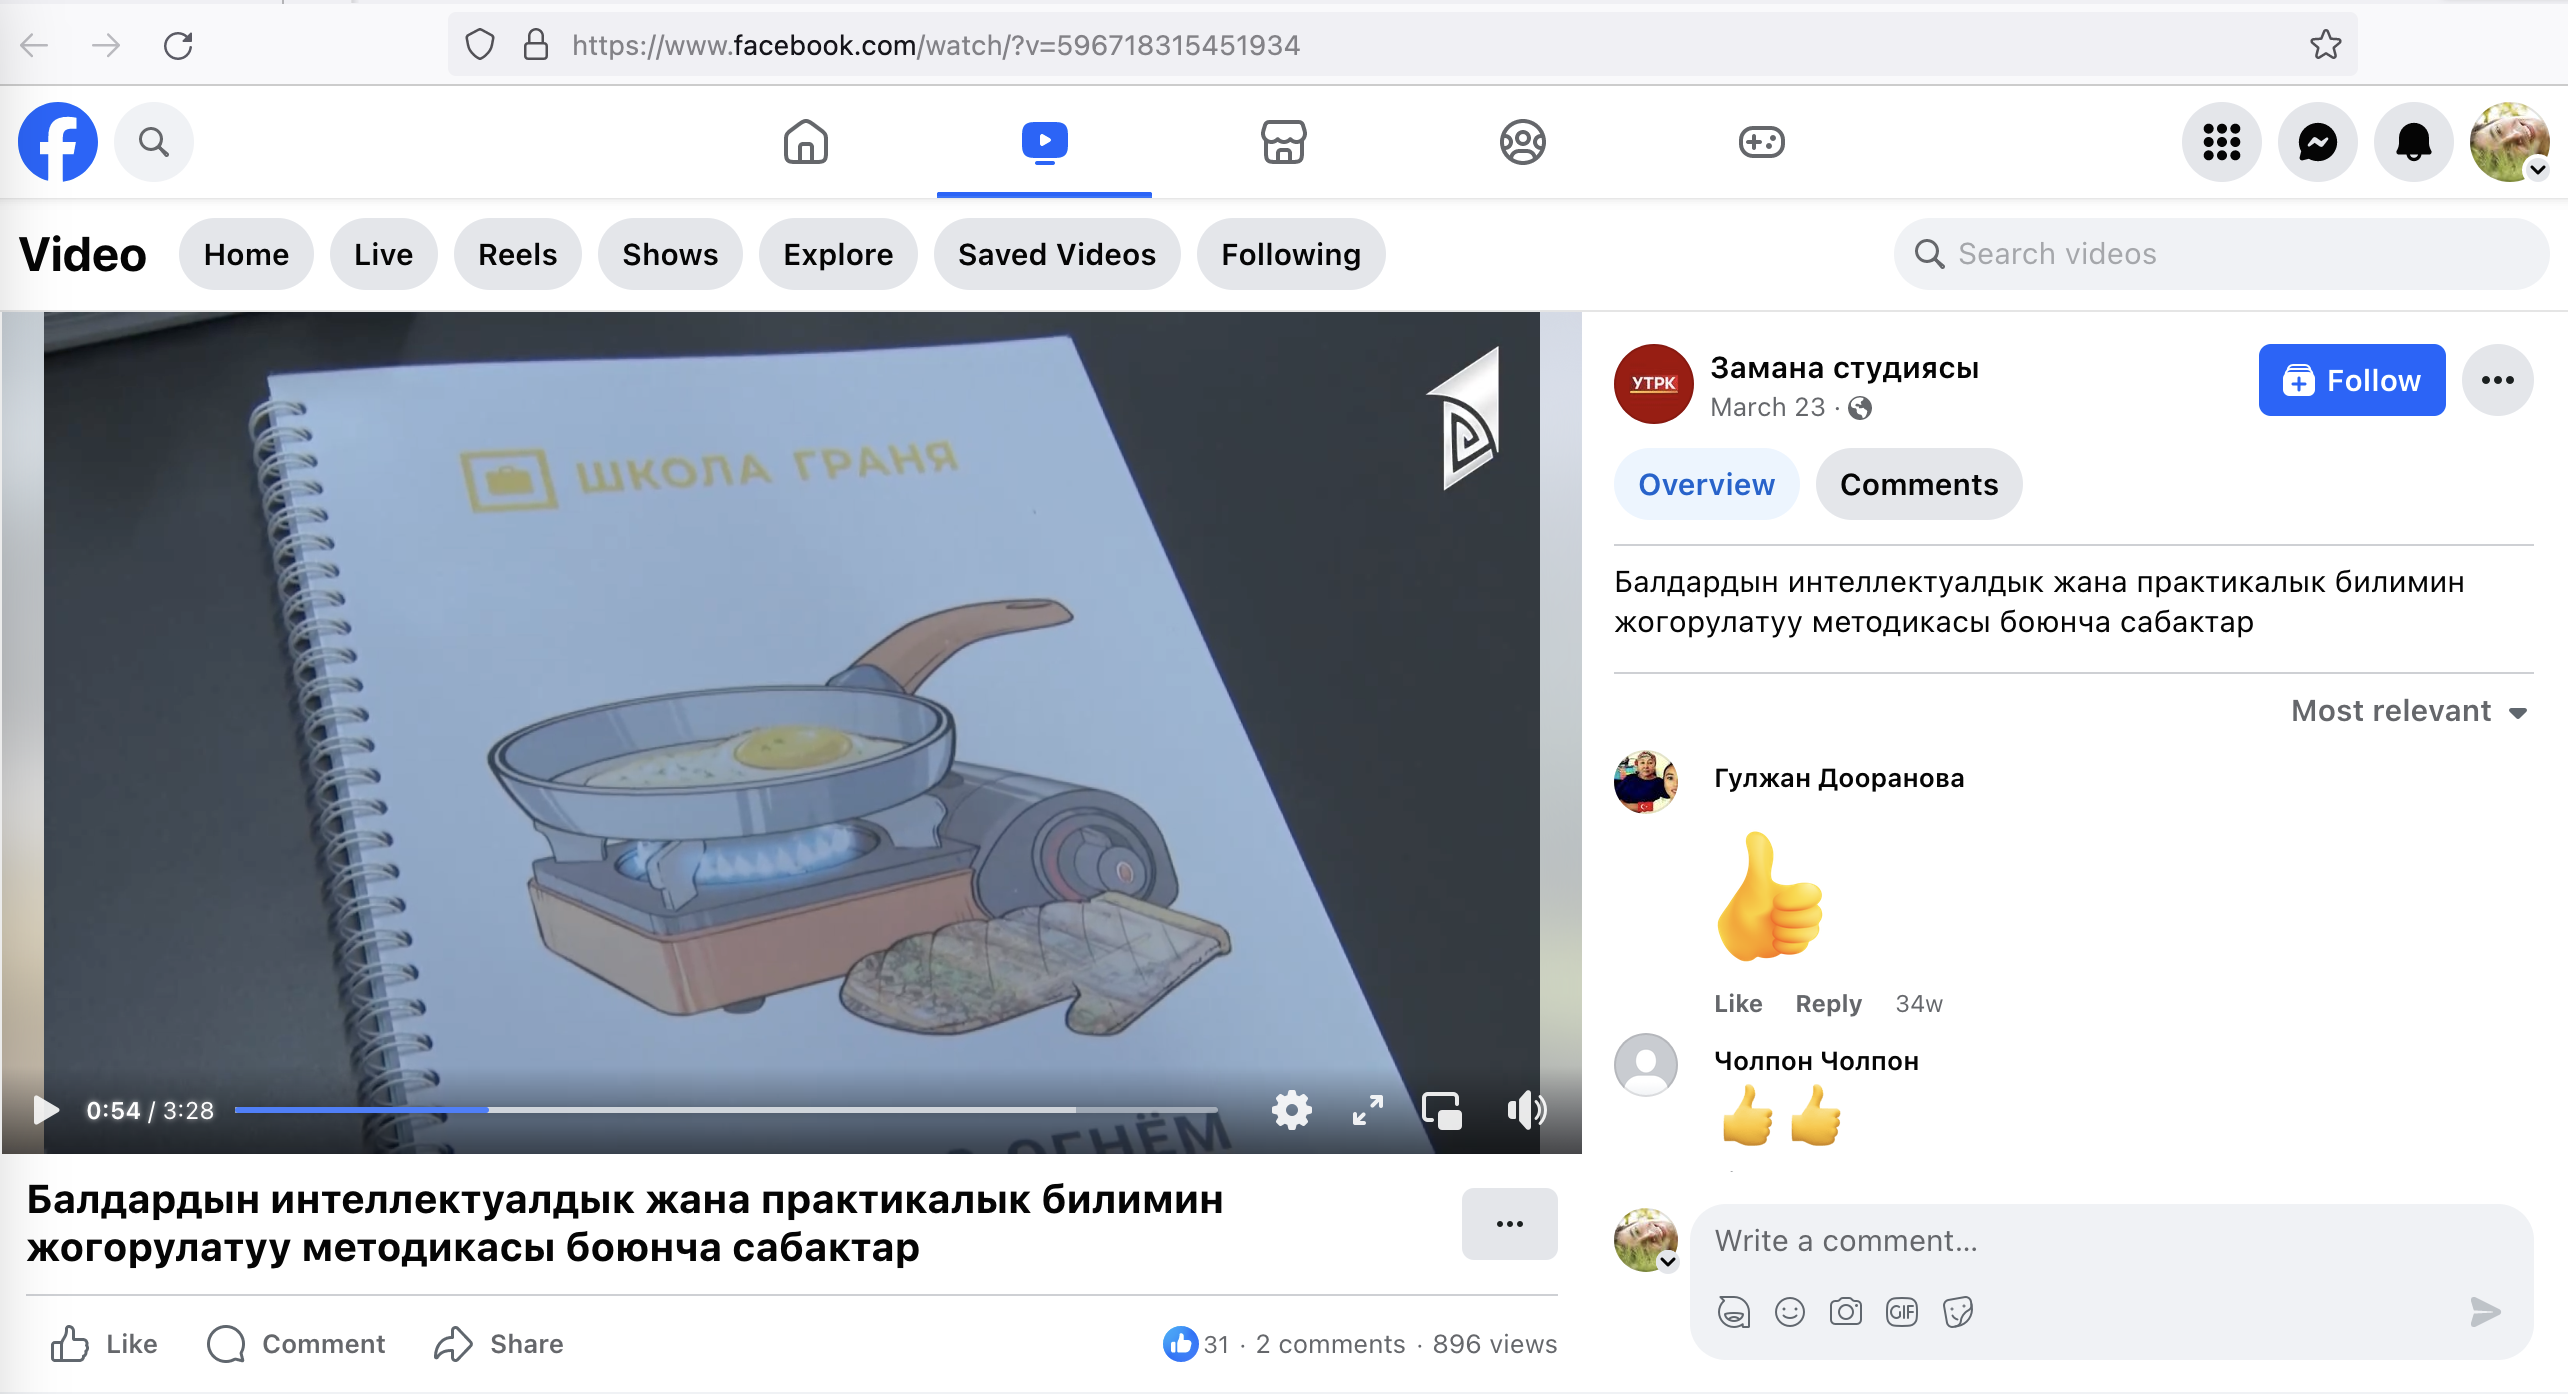
\includegraphics[width=\textwidth]{0_54_book-fire}

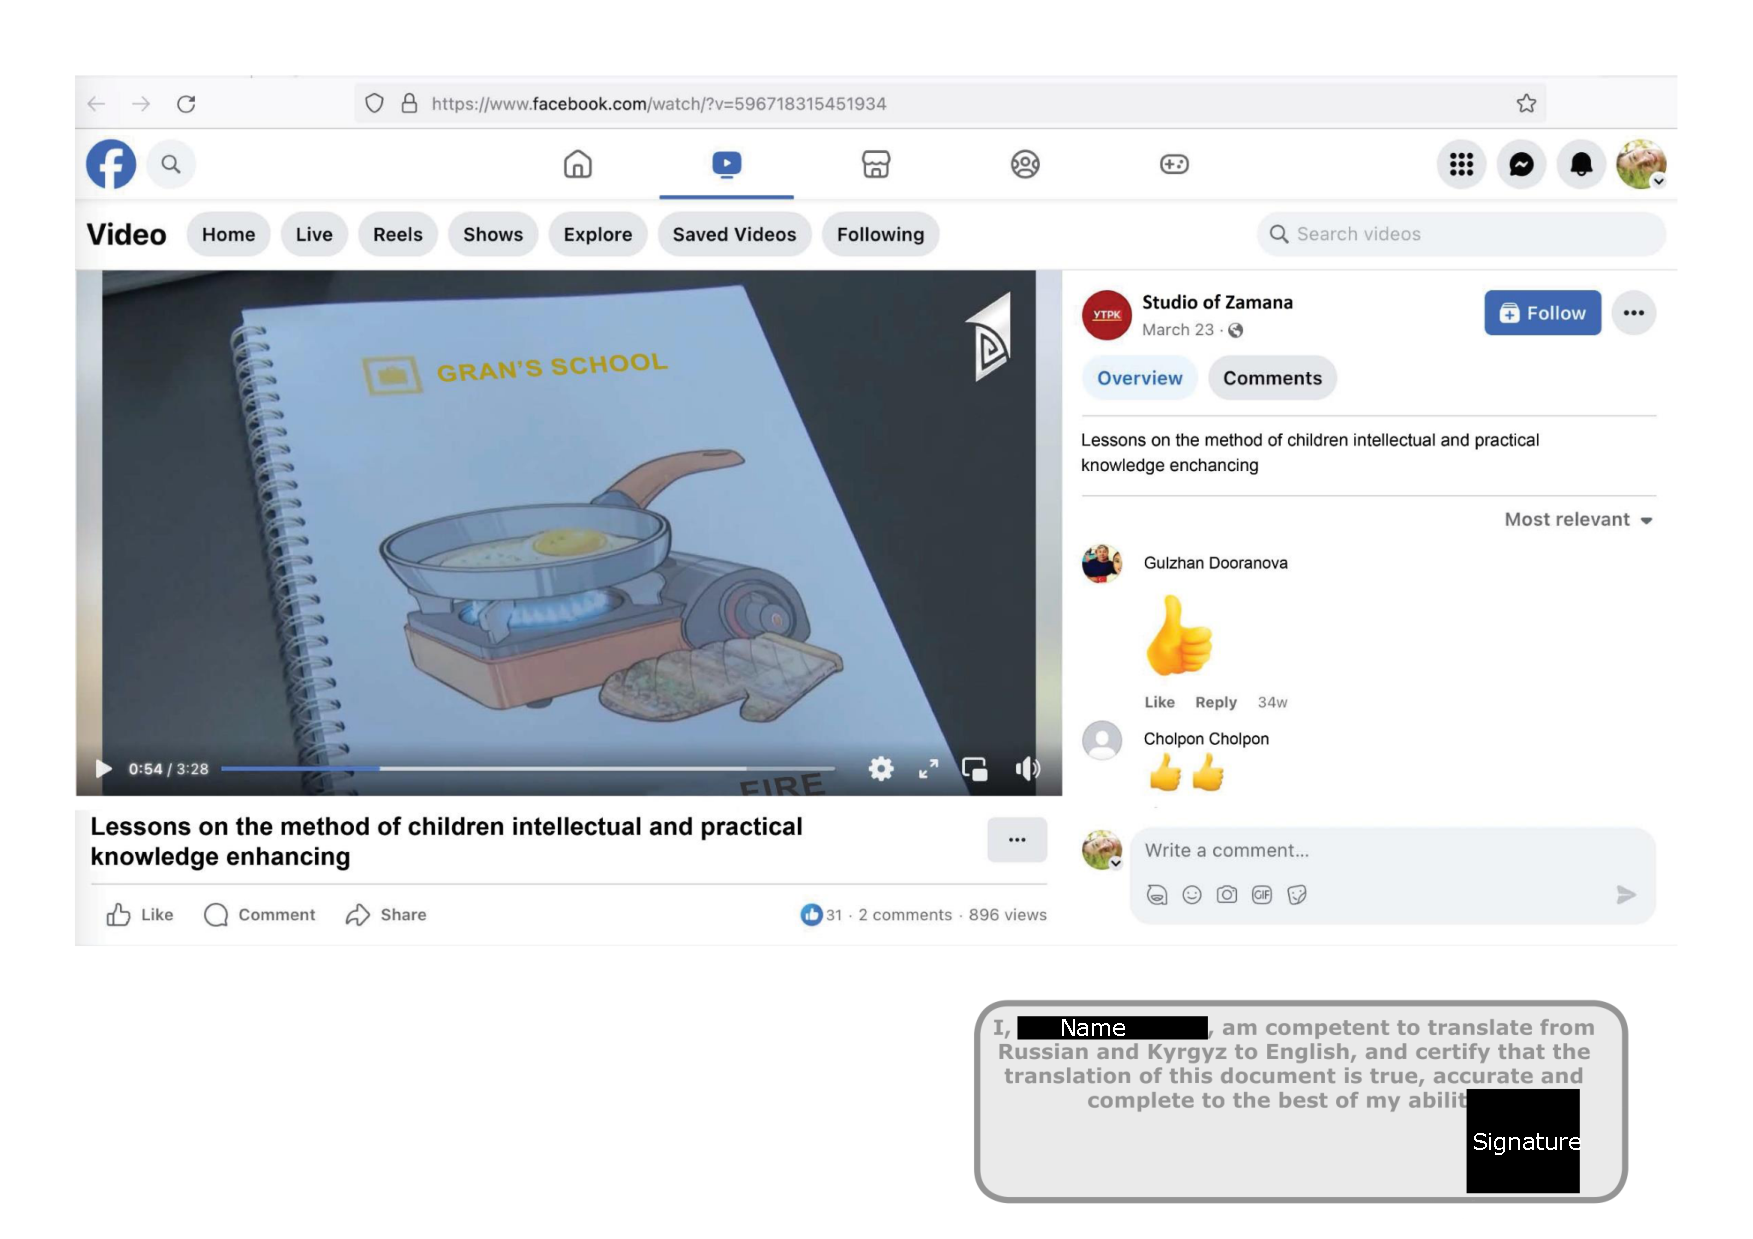
\includepdf[pages=-,angle=90]{0_54_book-fire_en_public}

This screenshot shows that the group has 78 thousand followers.
It also shows a link to the website of the channel, which supports authenticity:

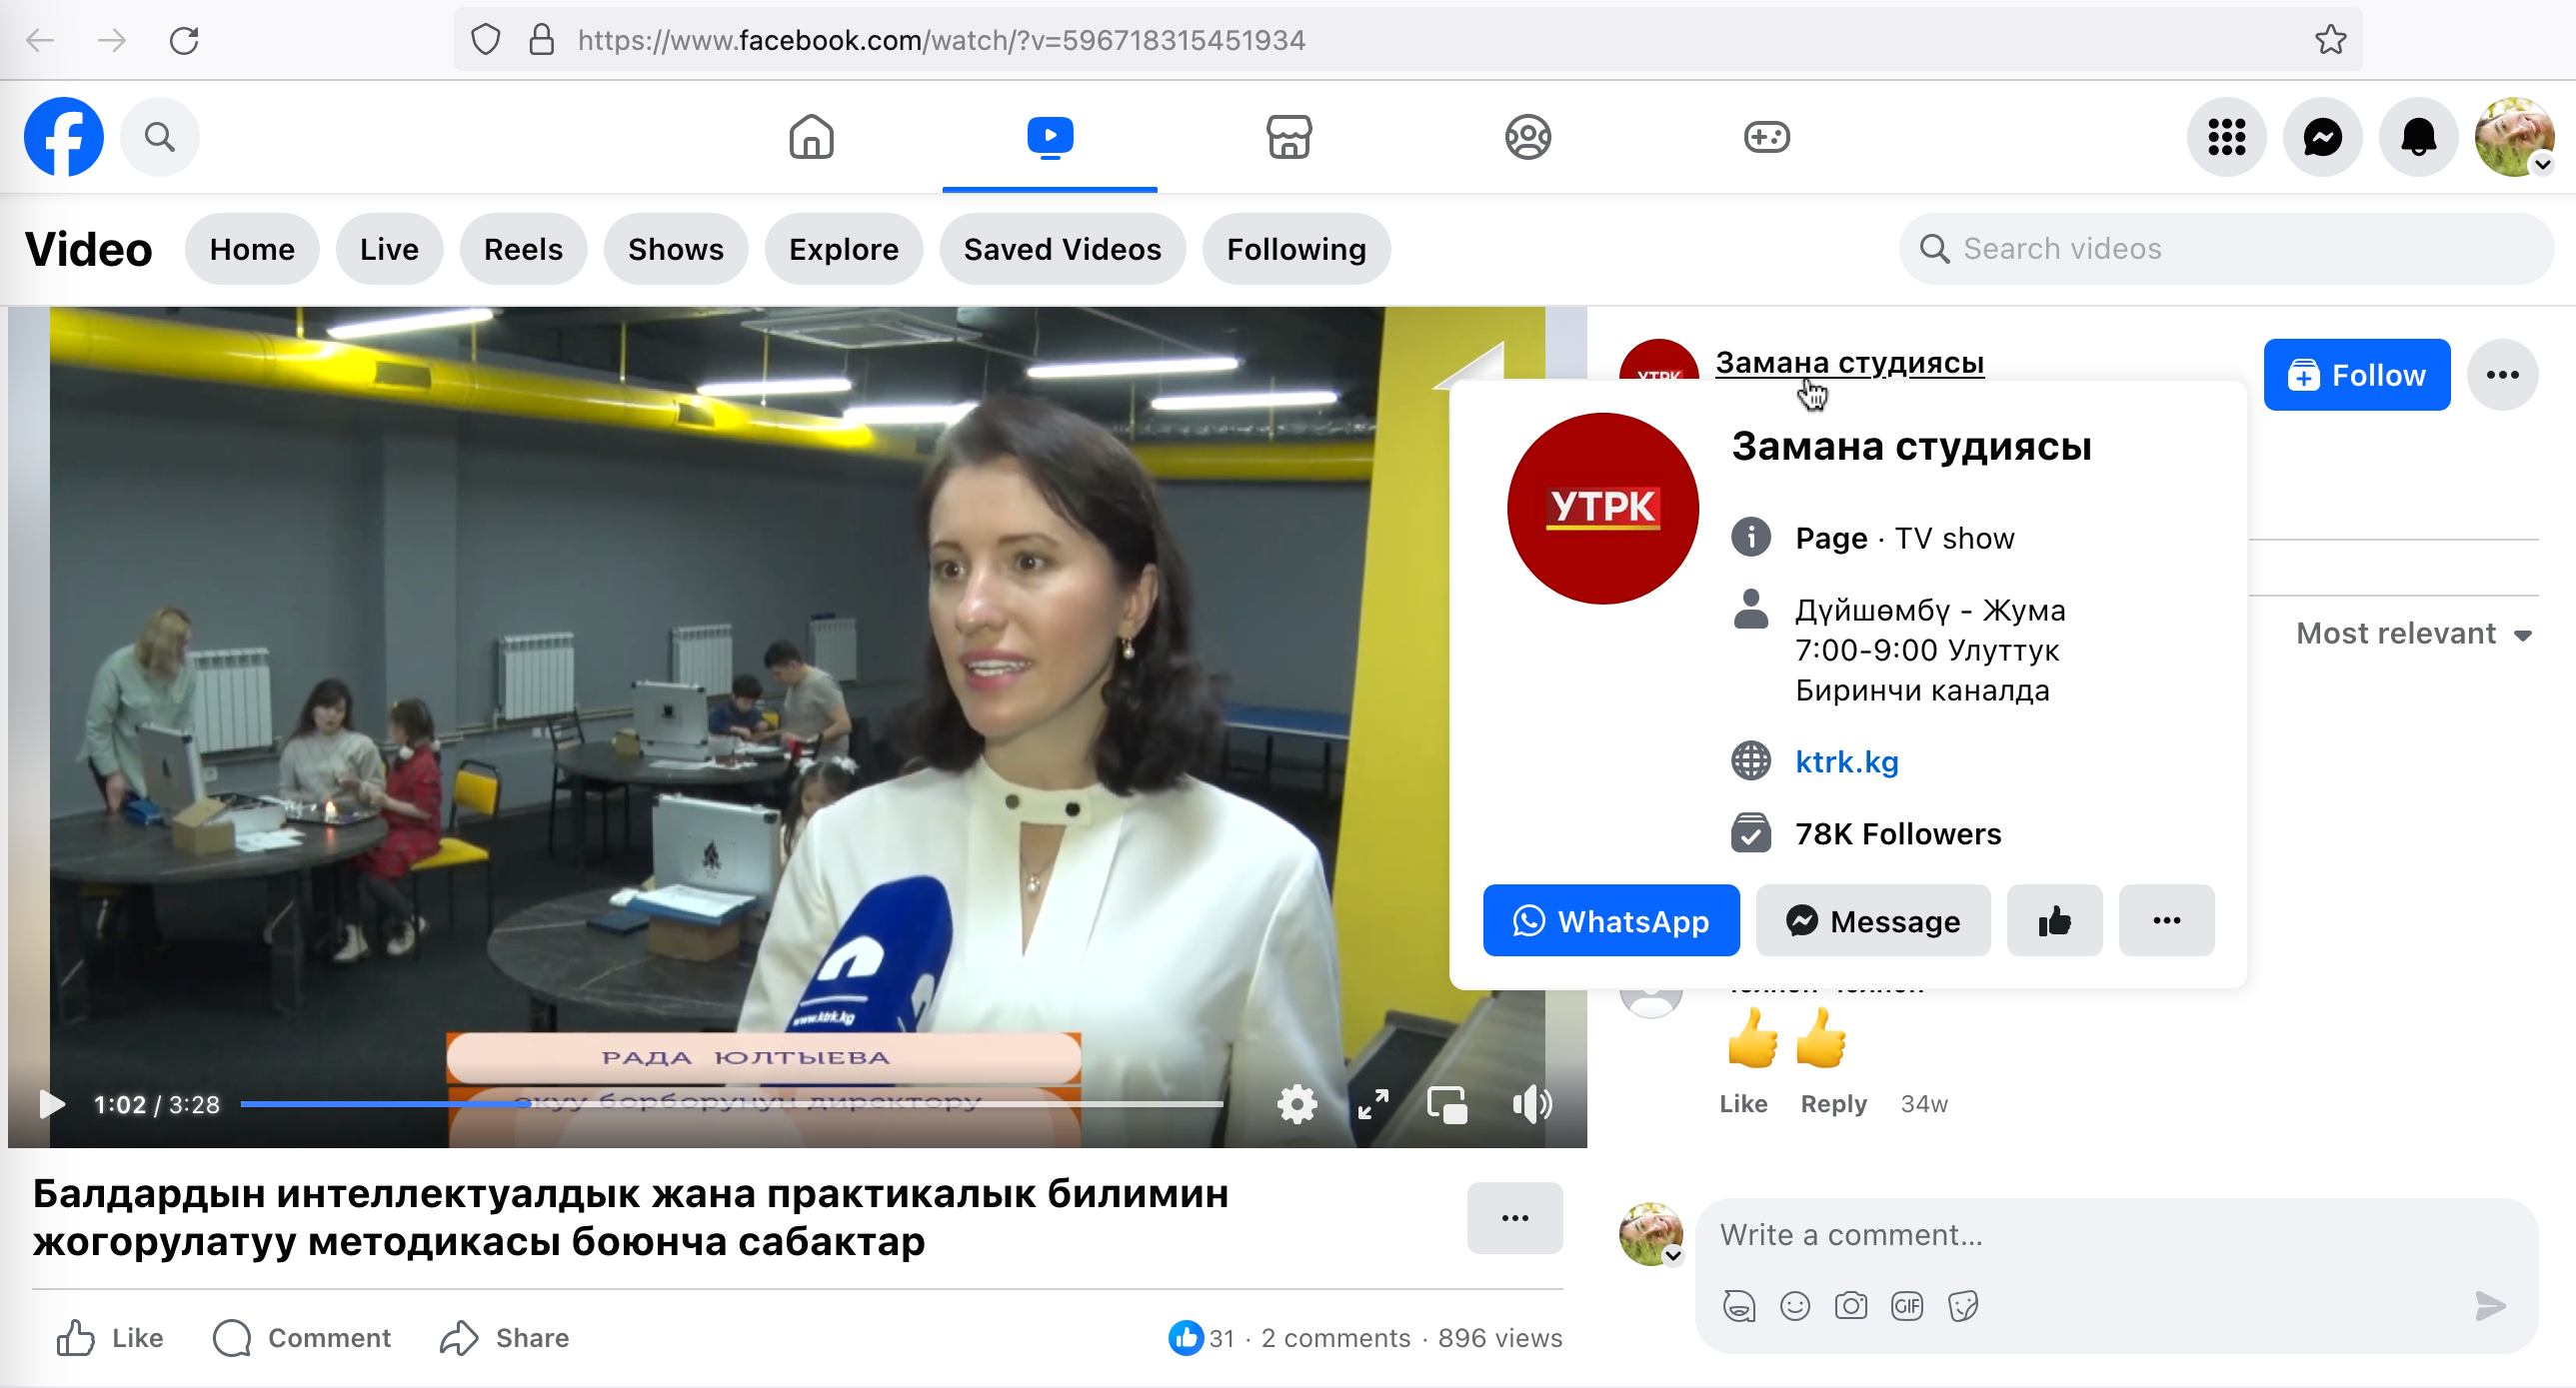
\includegraphics[width=\textwidth]{1_02_rada-stats}

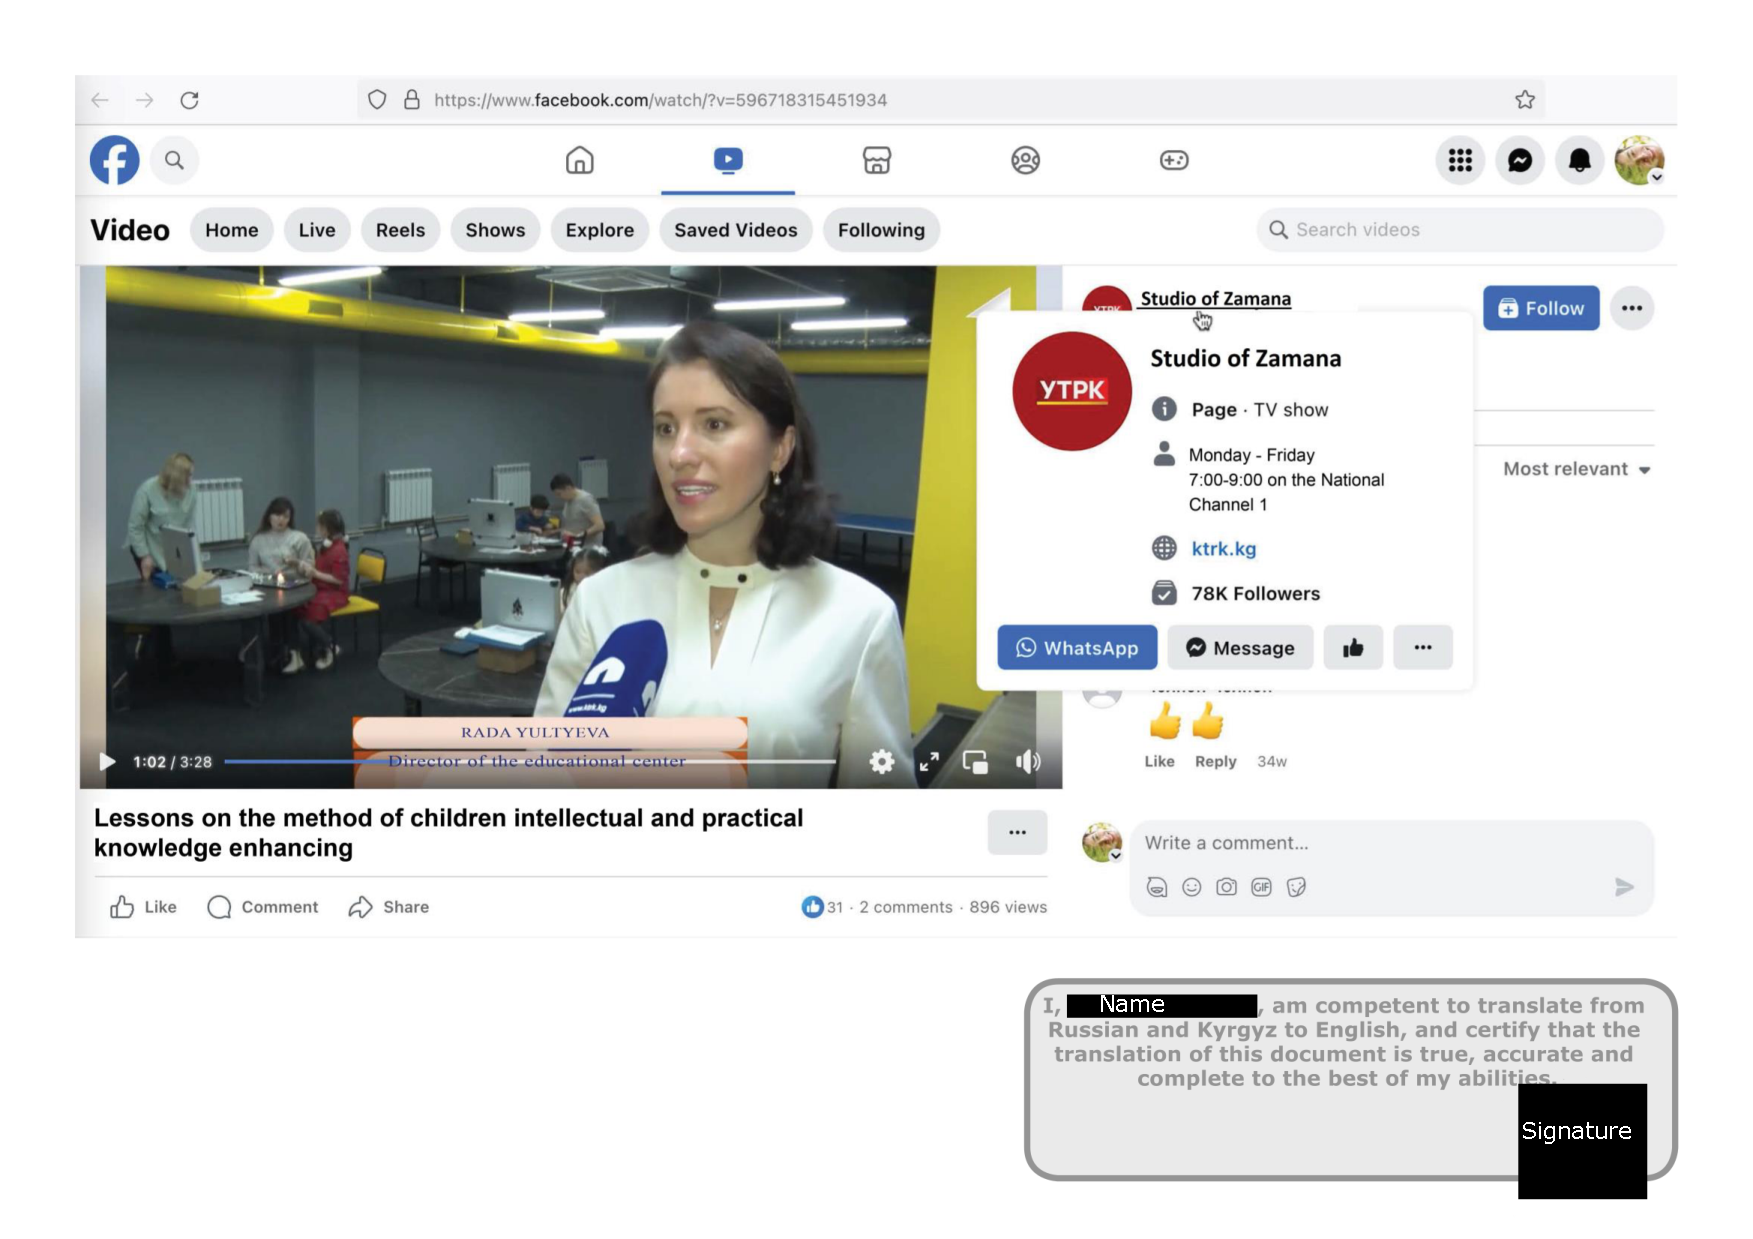
\includepdf[pages=-,angle=90]{1_02_rada-stats_en_public}

At 2:30, the microphone with `ktrk.kg' address is visible, which also supports authenticity:

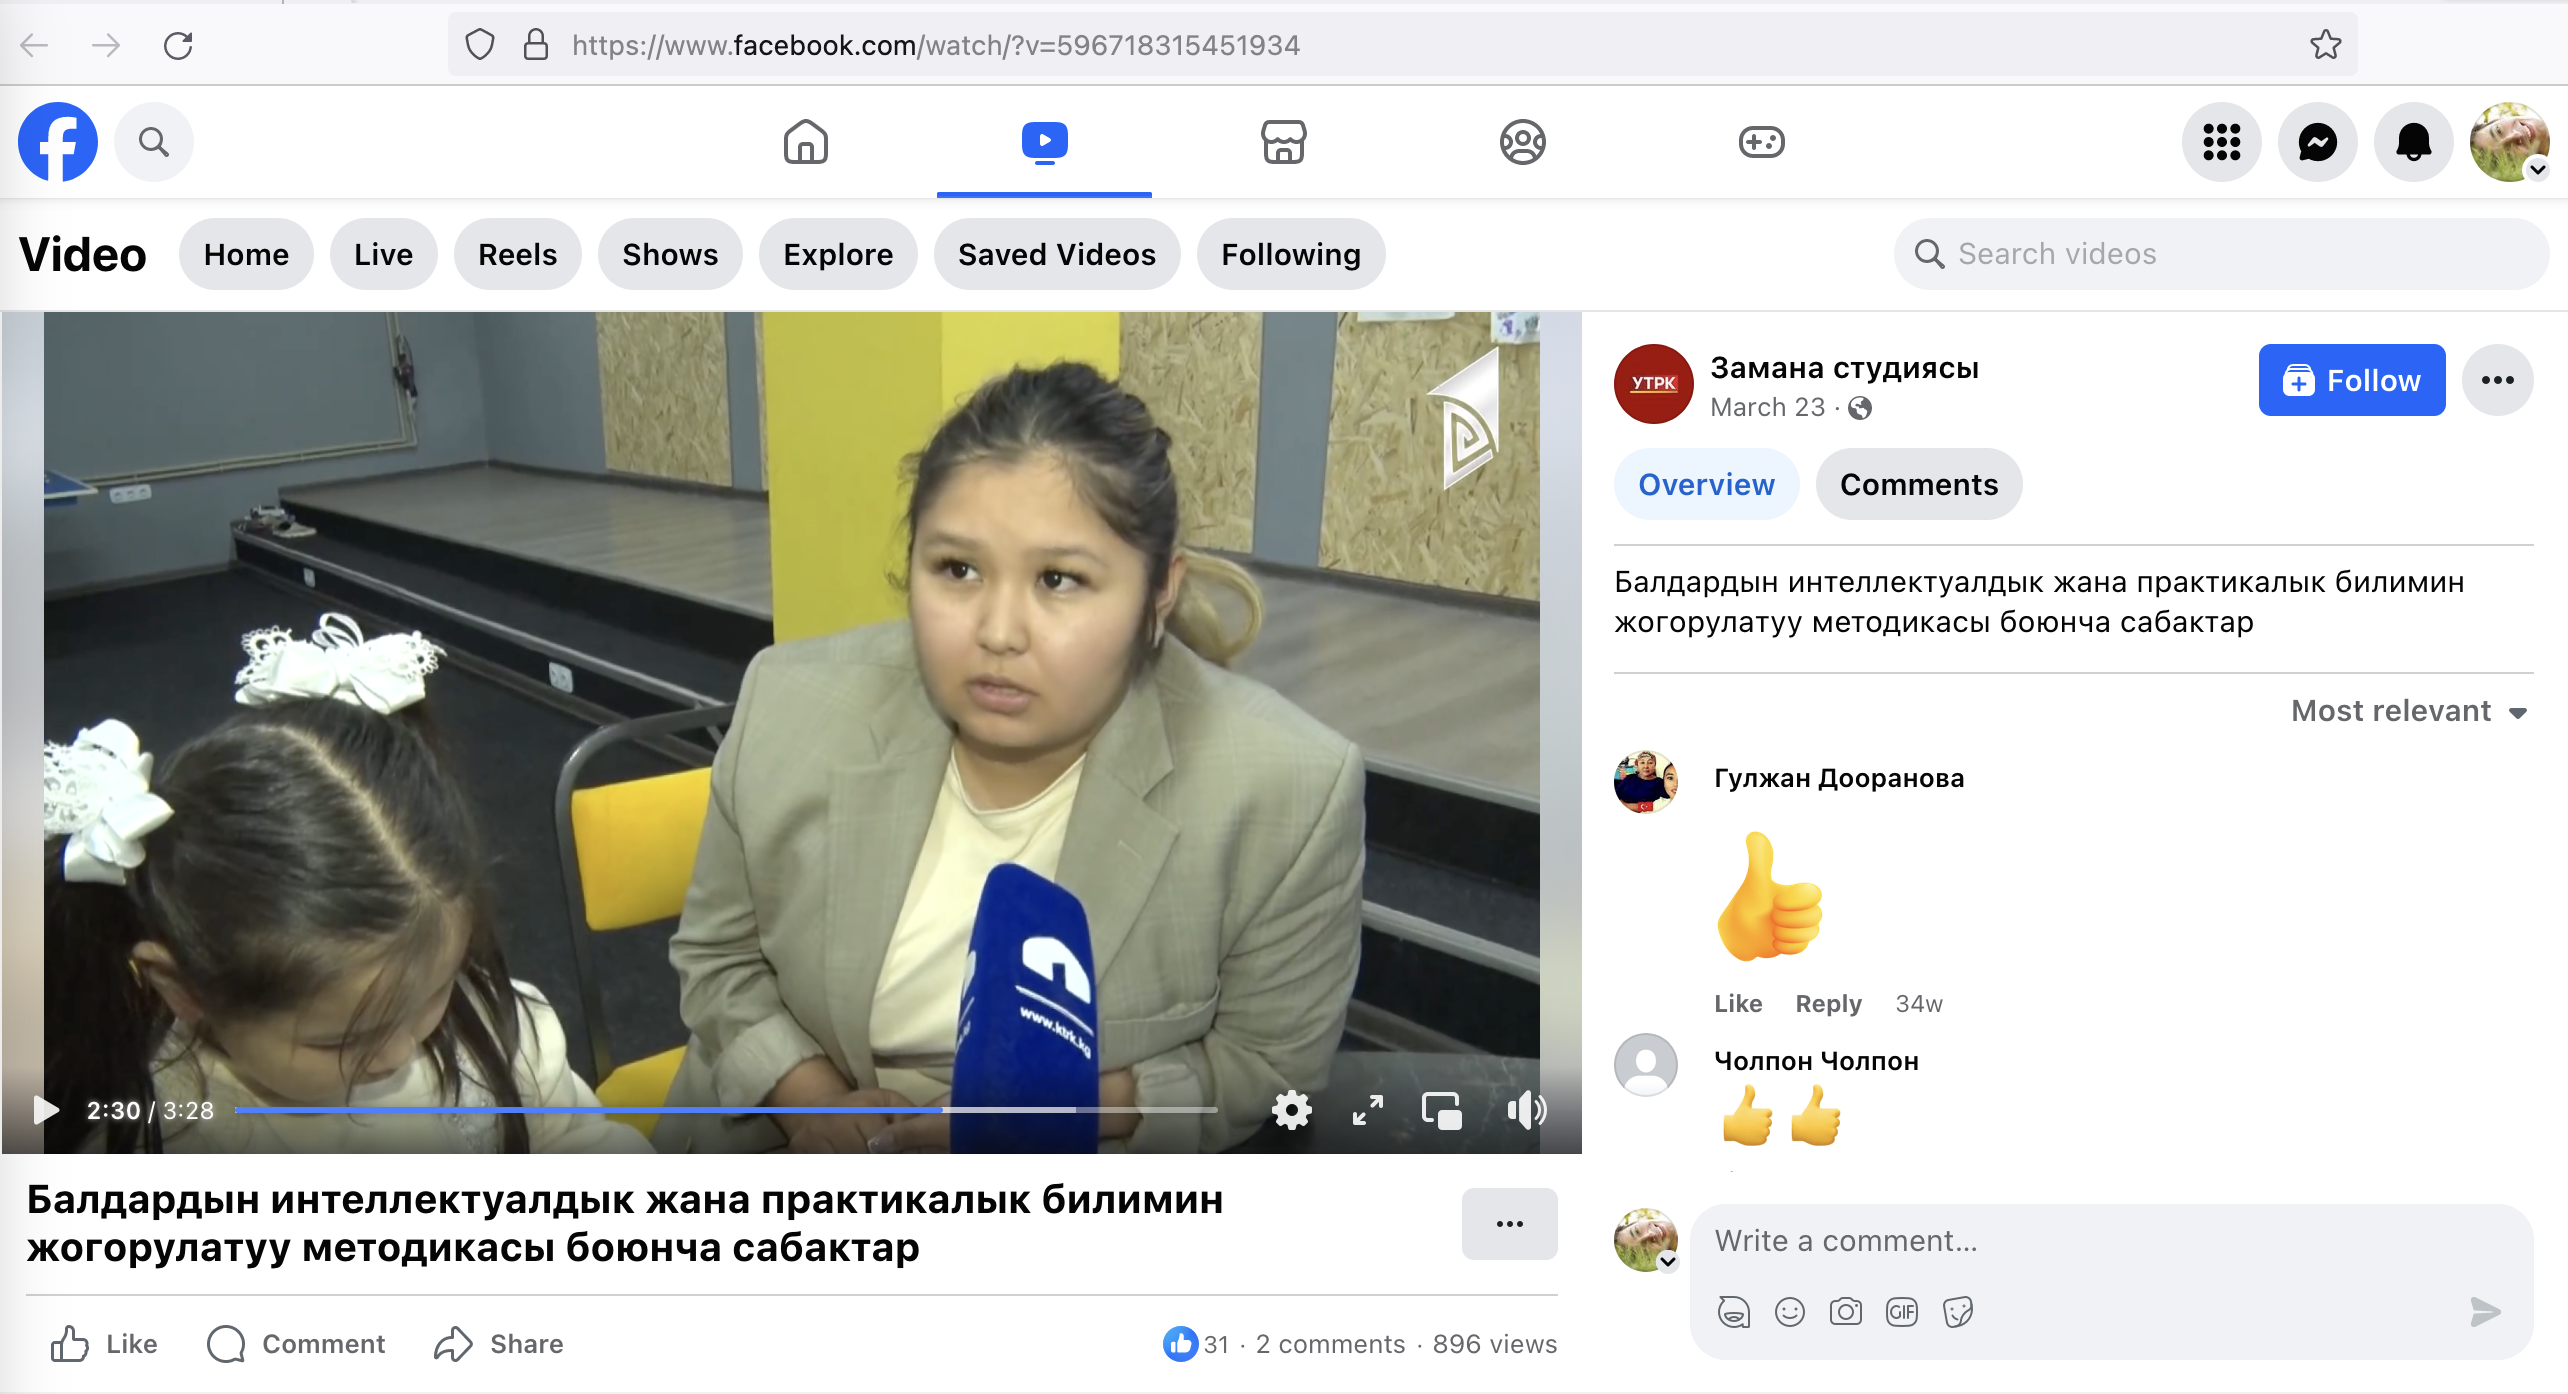
\includegraphics[width=\textwidth]{2_30_girls}

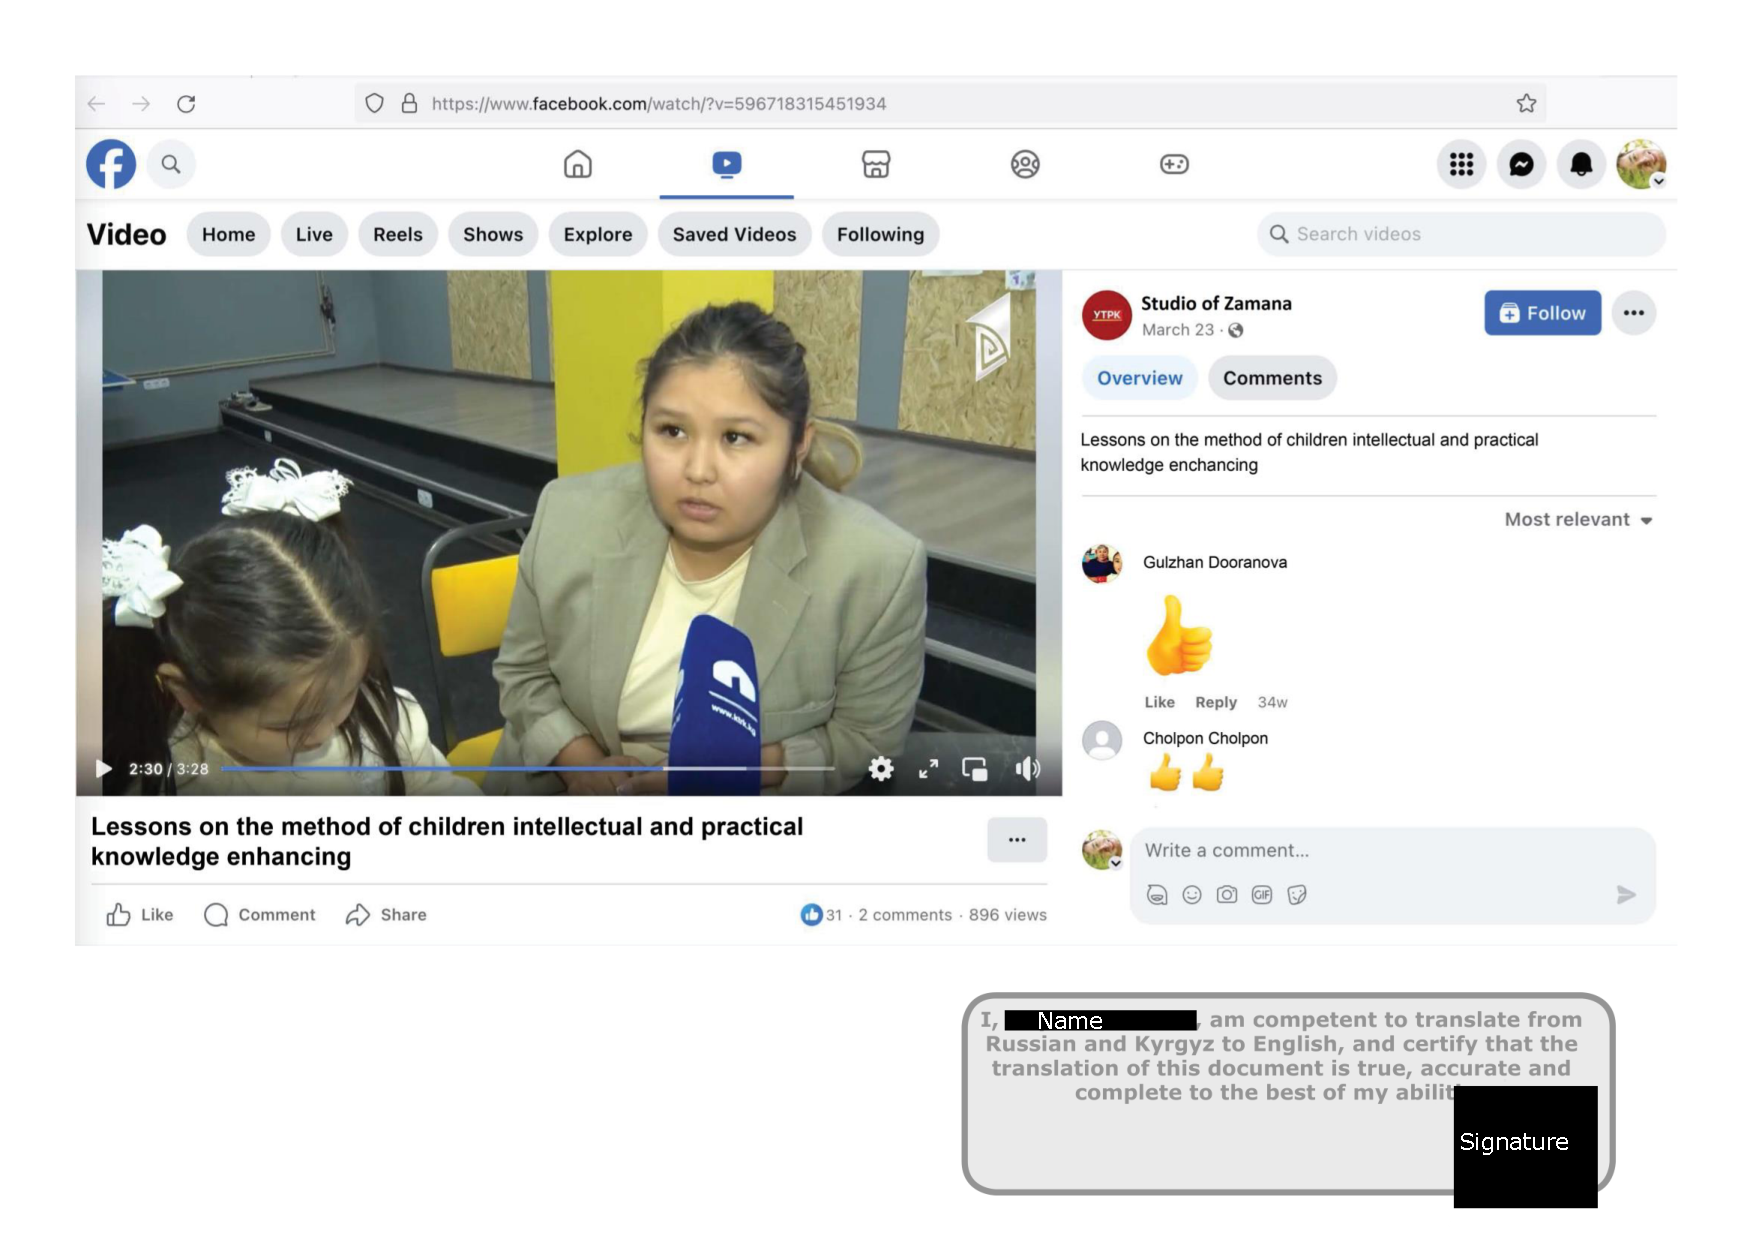
\includepdf[pages=-,angle=90]{2_30_girls_en_public}

At 3:16, another textbook from `Gran's School' on working with clay is shown:

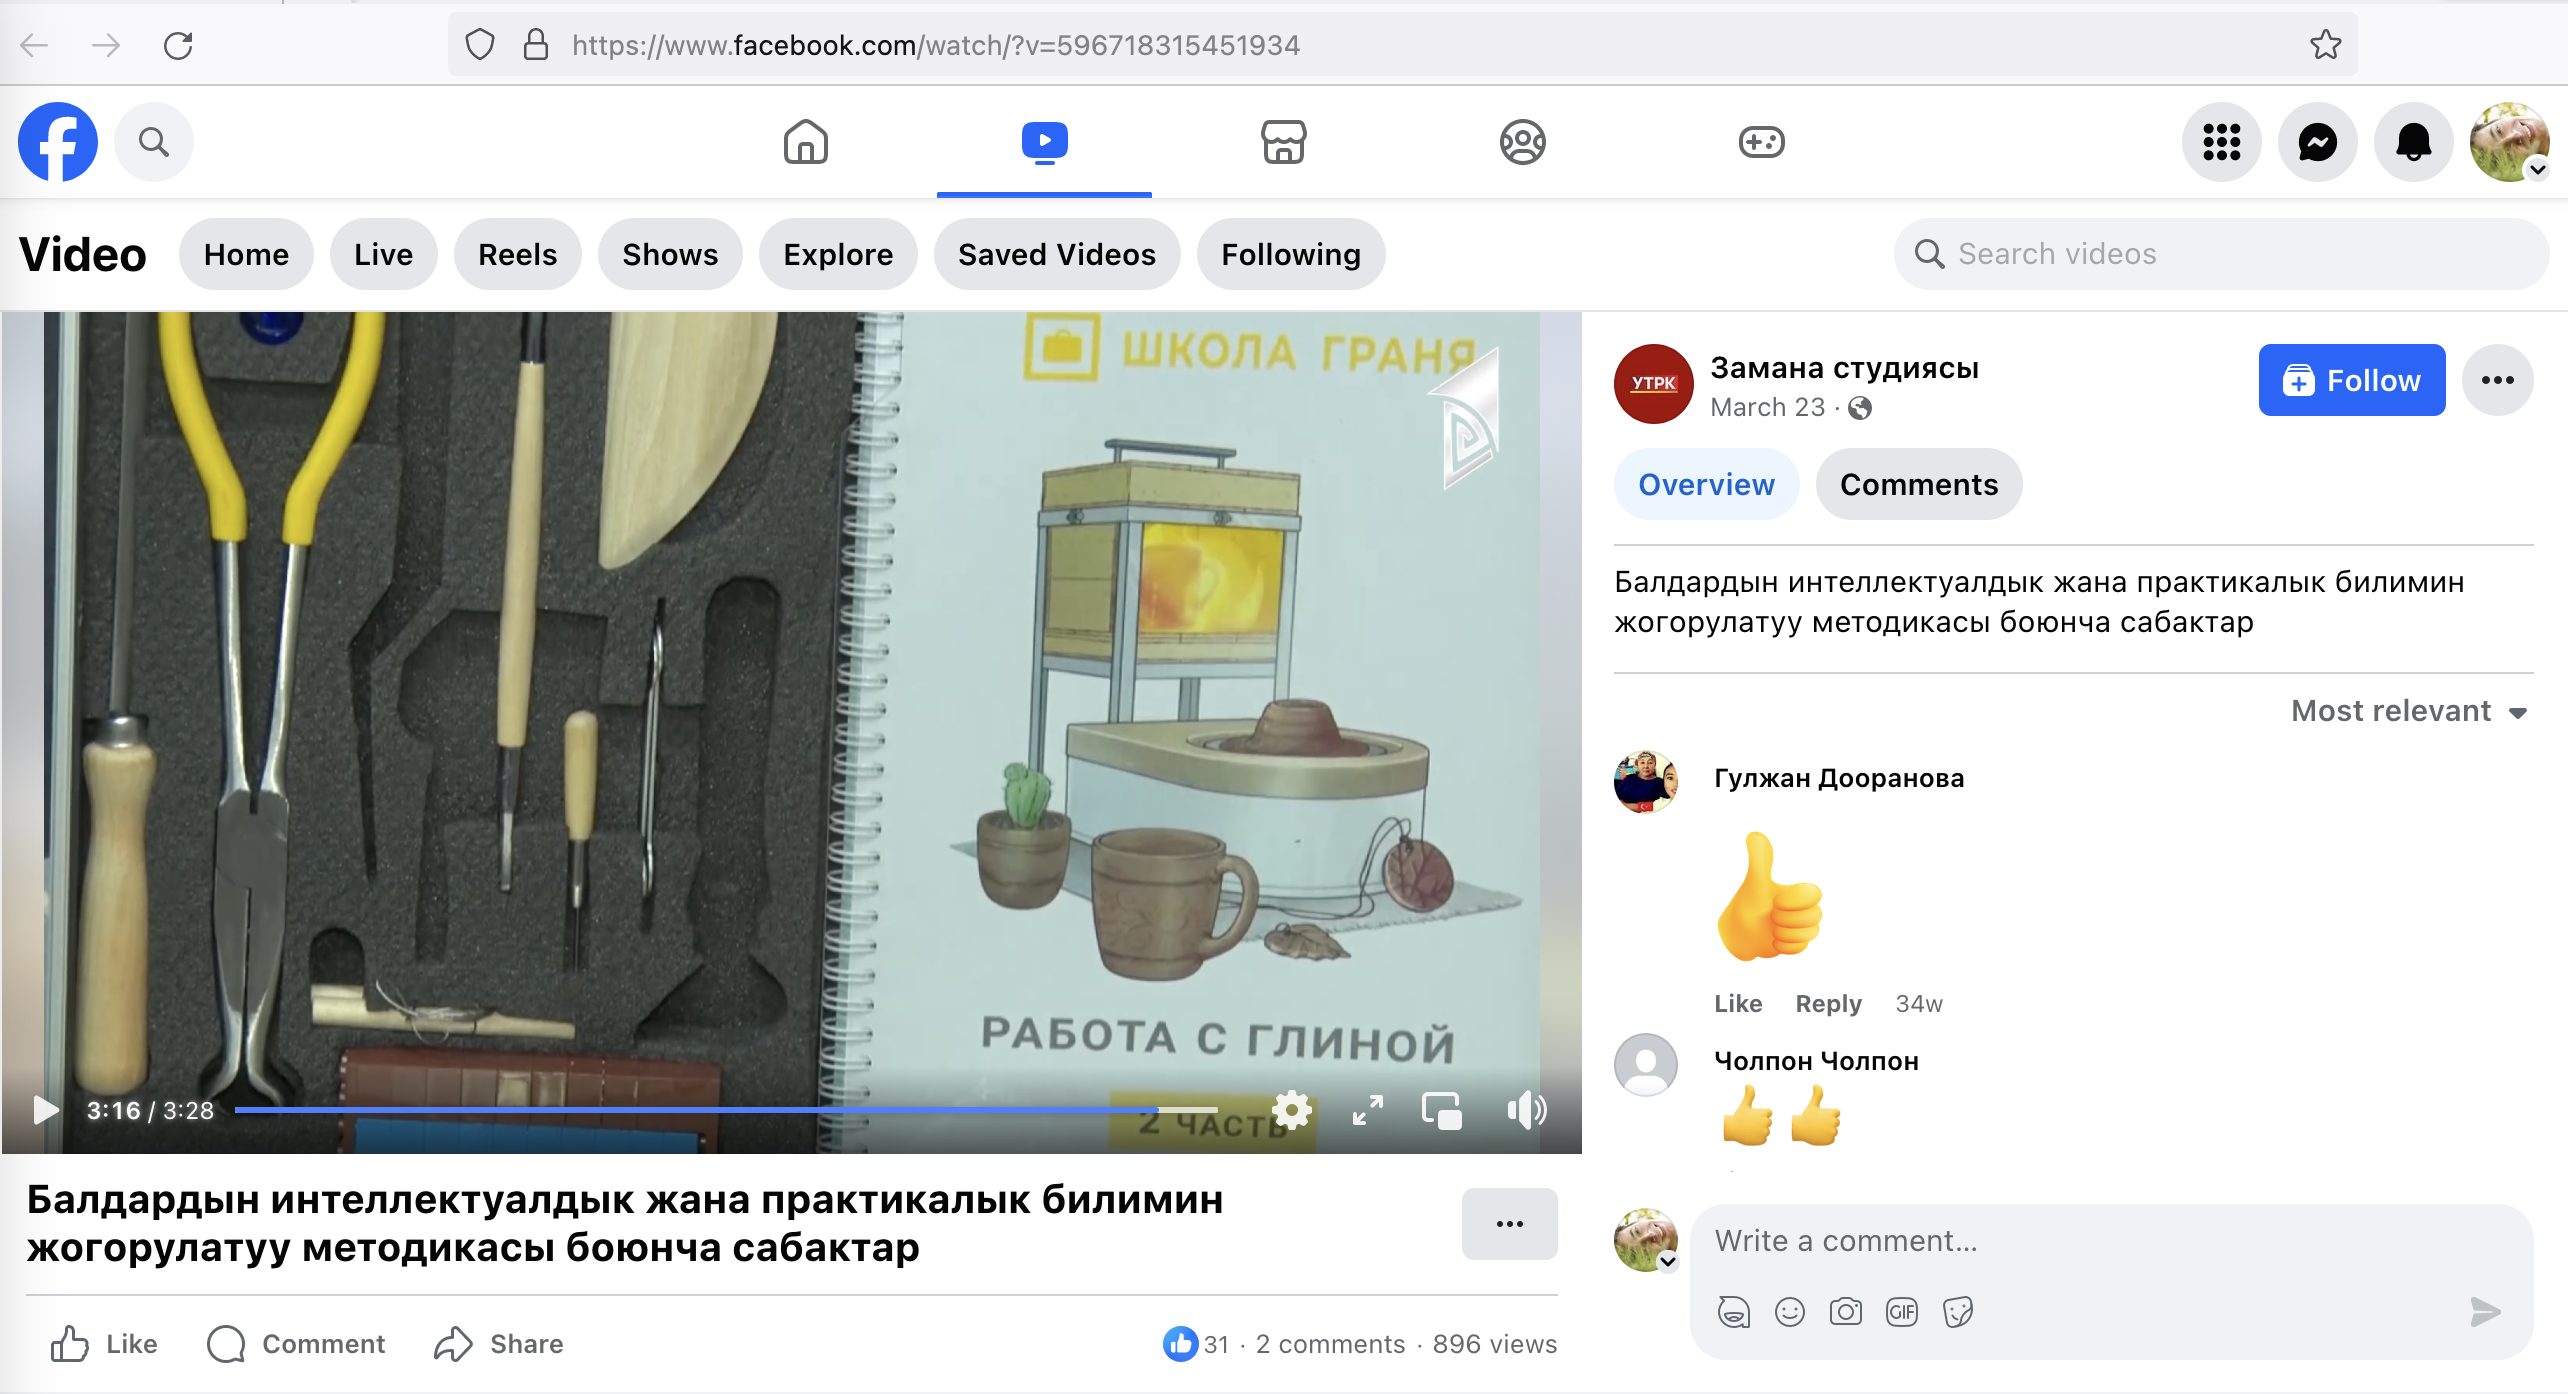
\includegraphics[width=\textwidth]{3_16_book-clay}

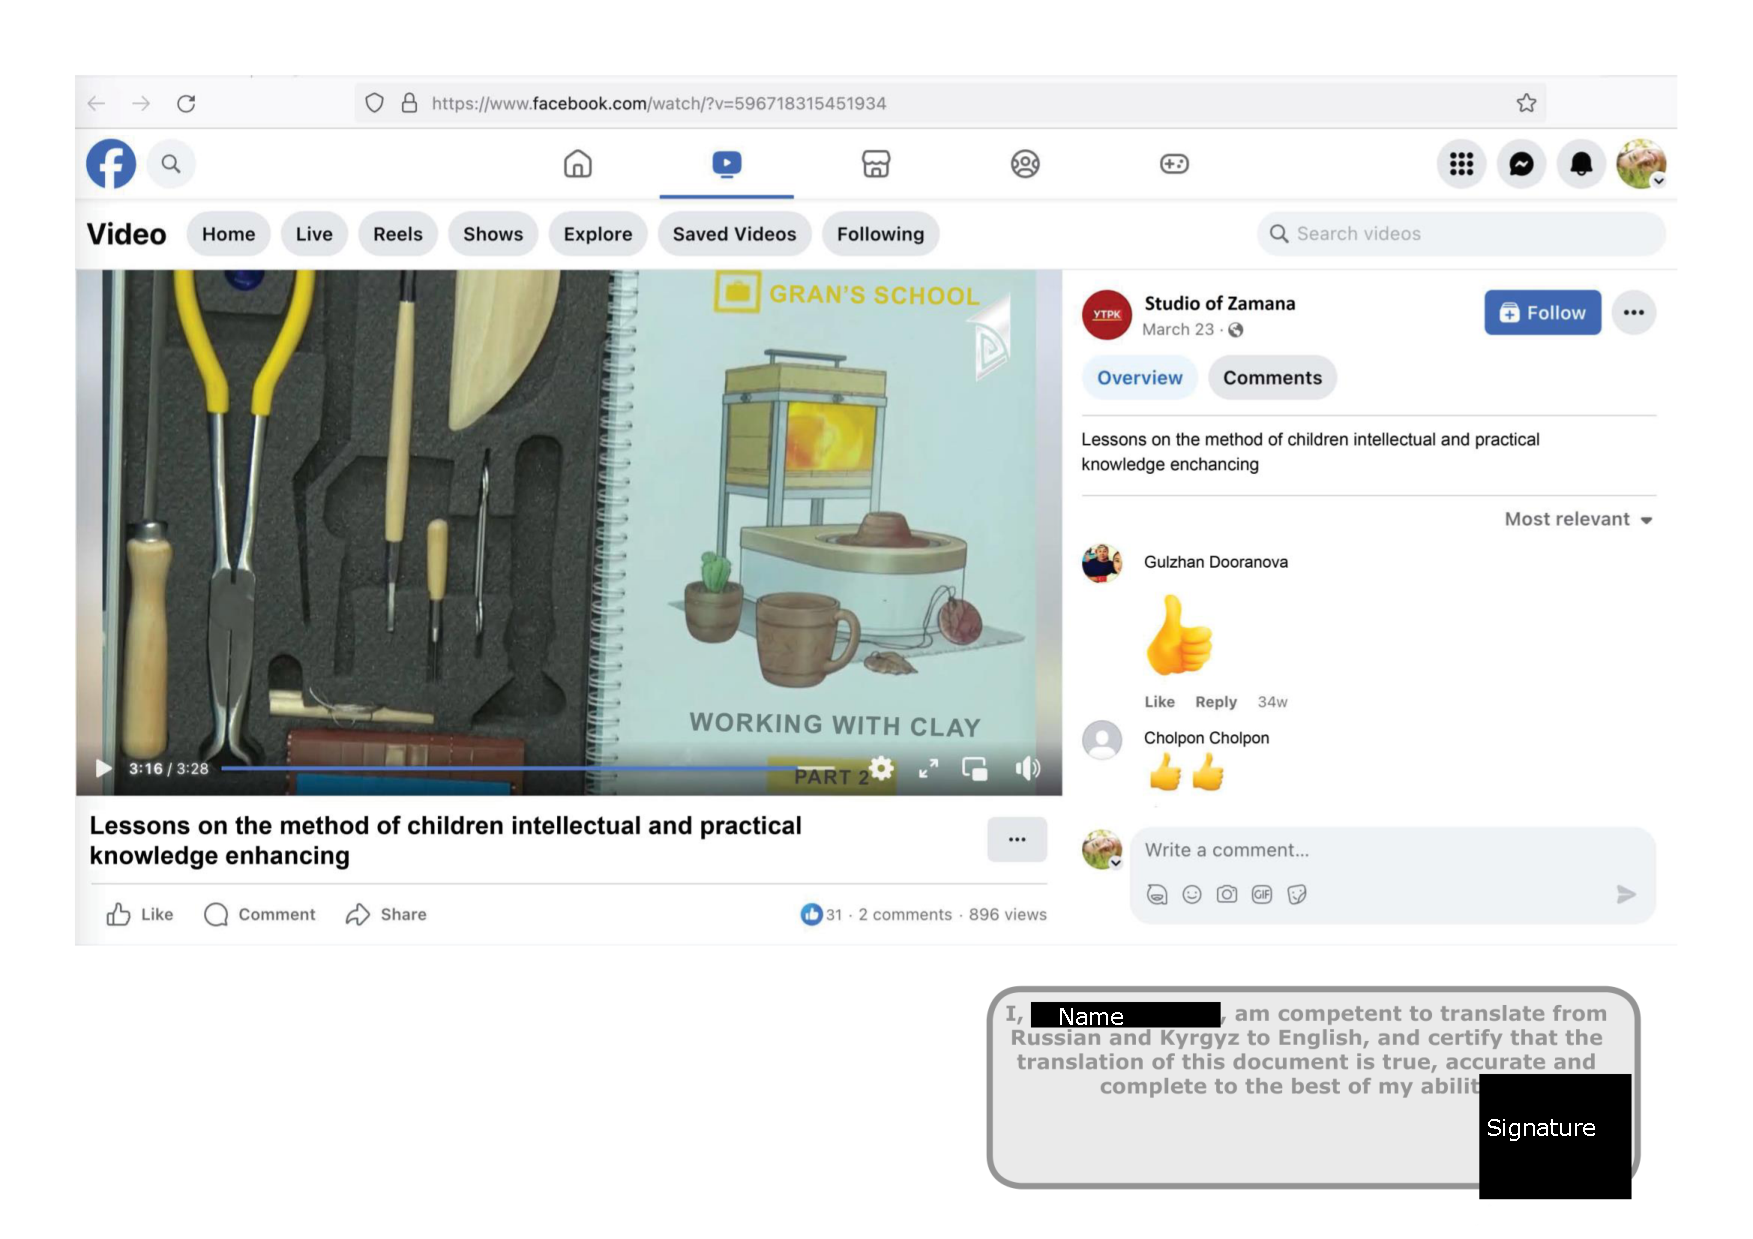
\includepdf[pages=-,angle=90]{3_16_book-clay_en_public}

At 3:28, three kits are displayed:

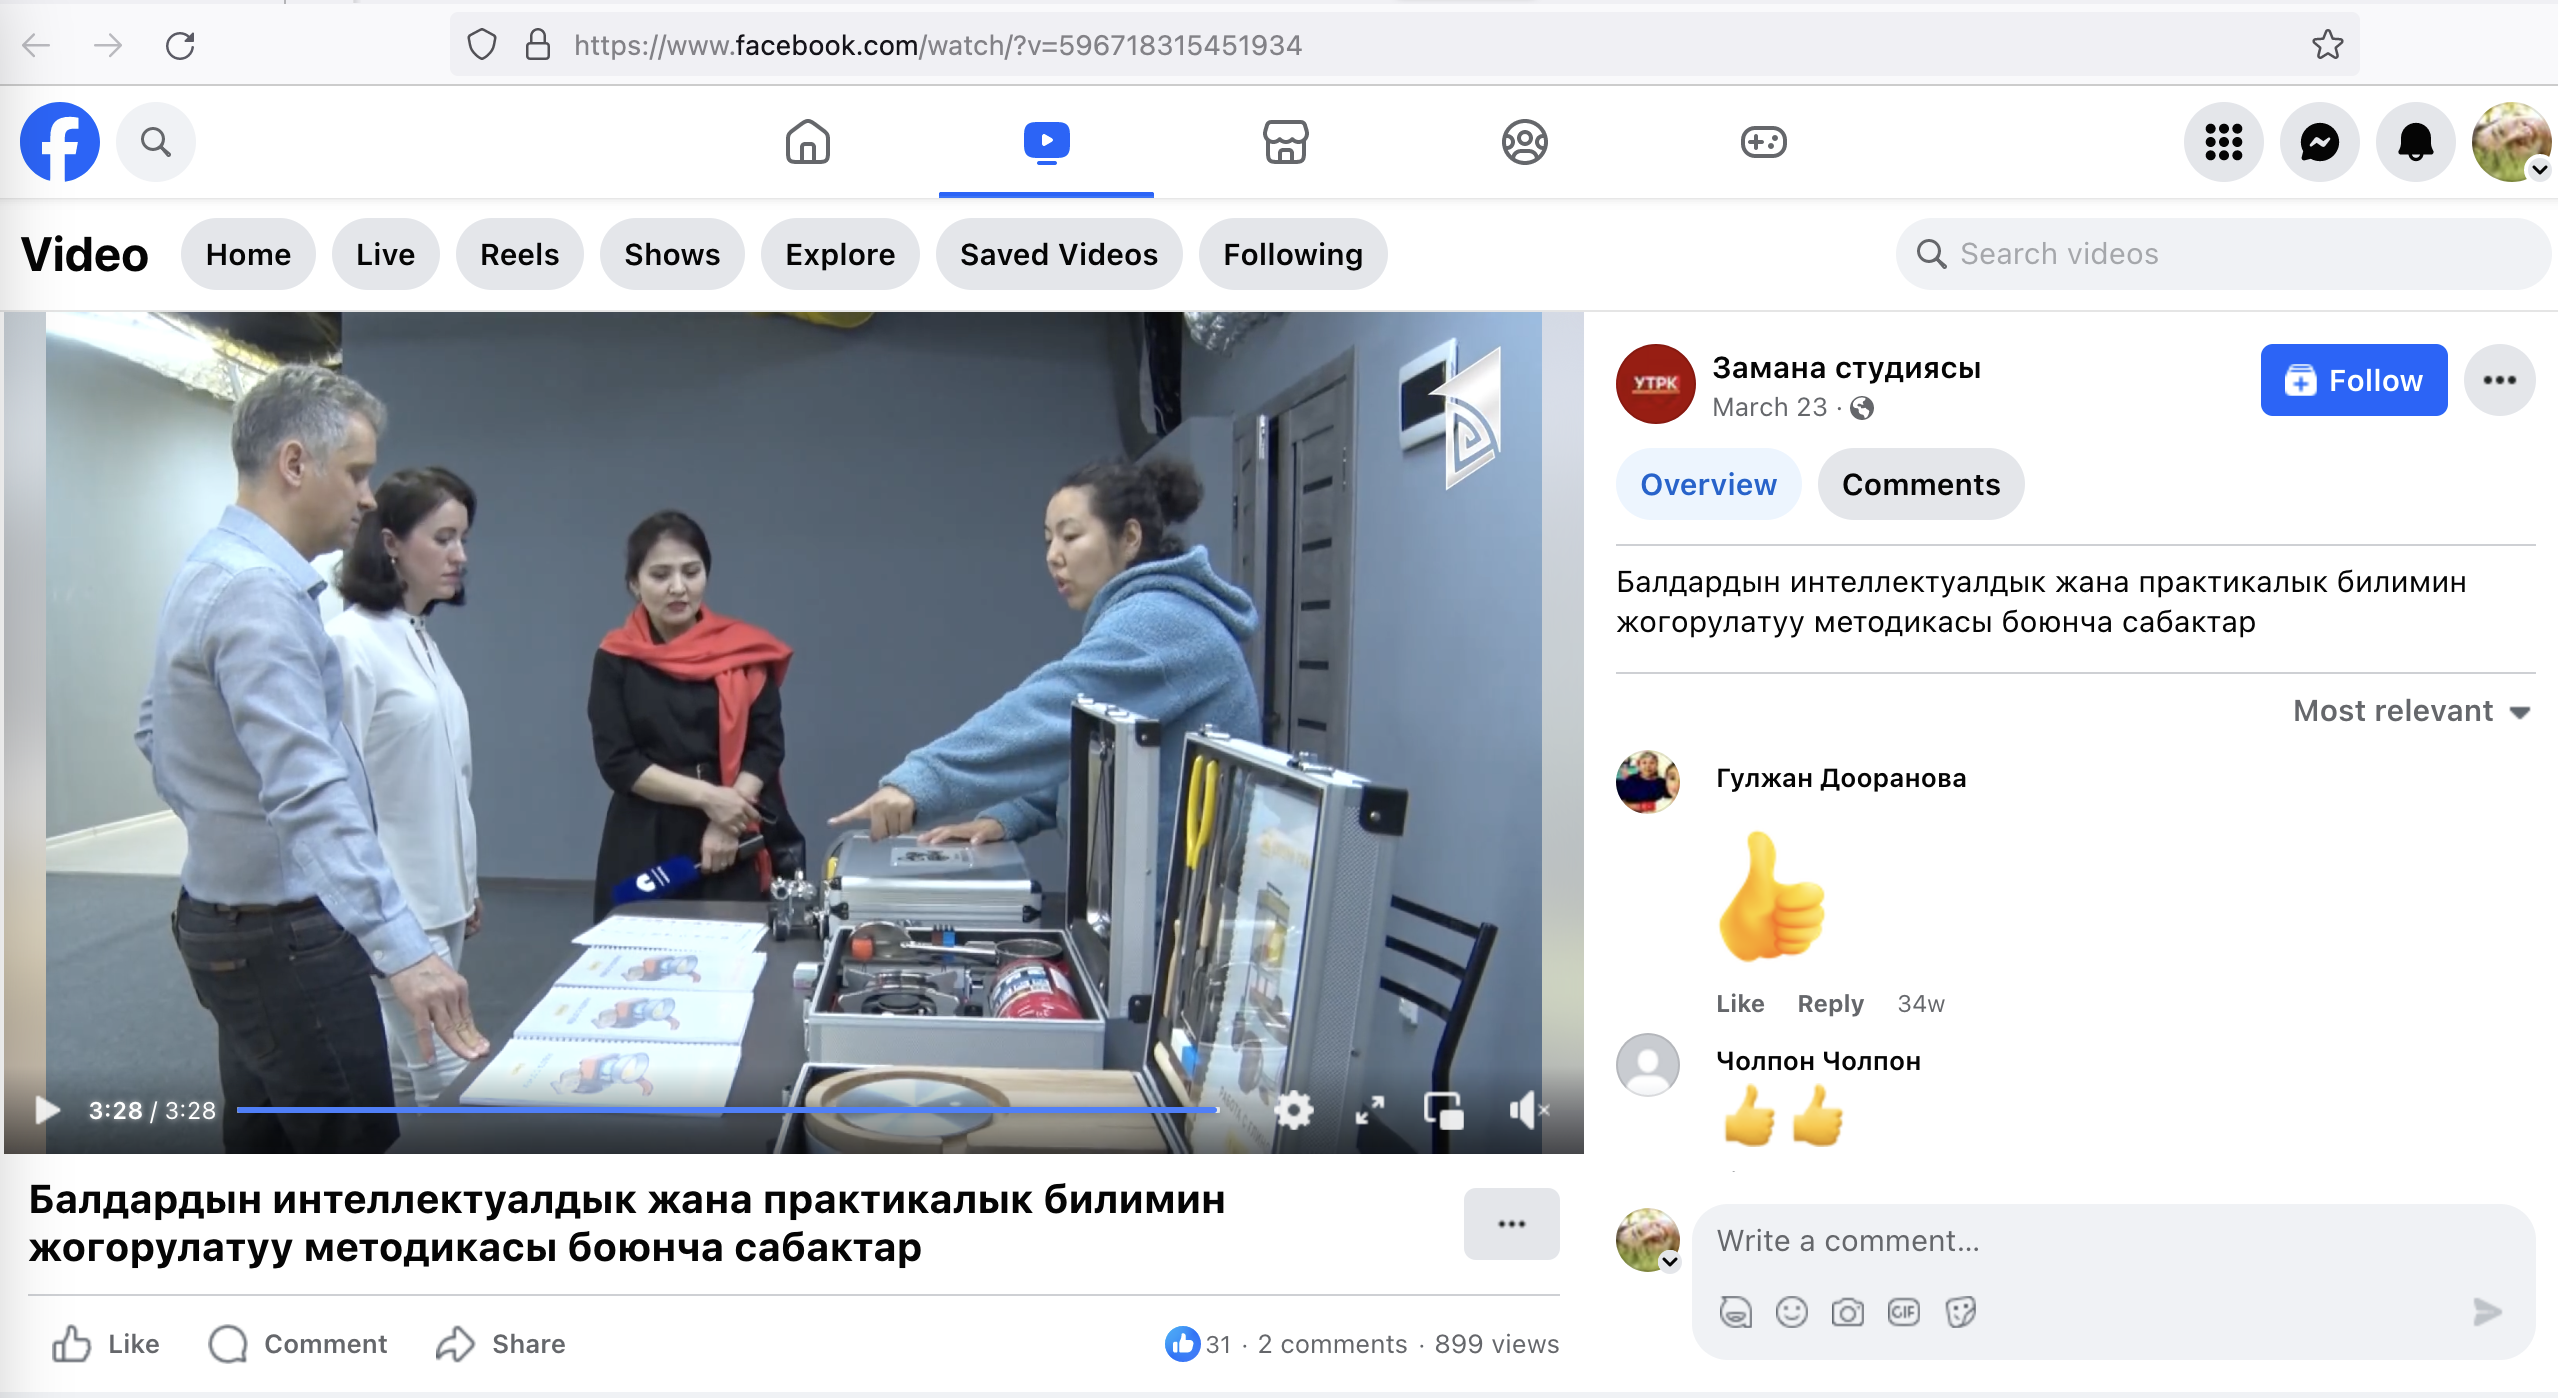
\includegraphics[width=\textwidth]{3_28_stand}

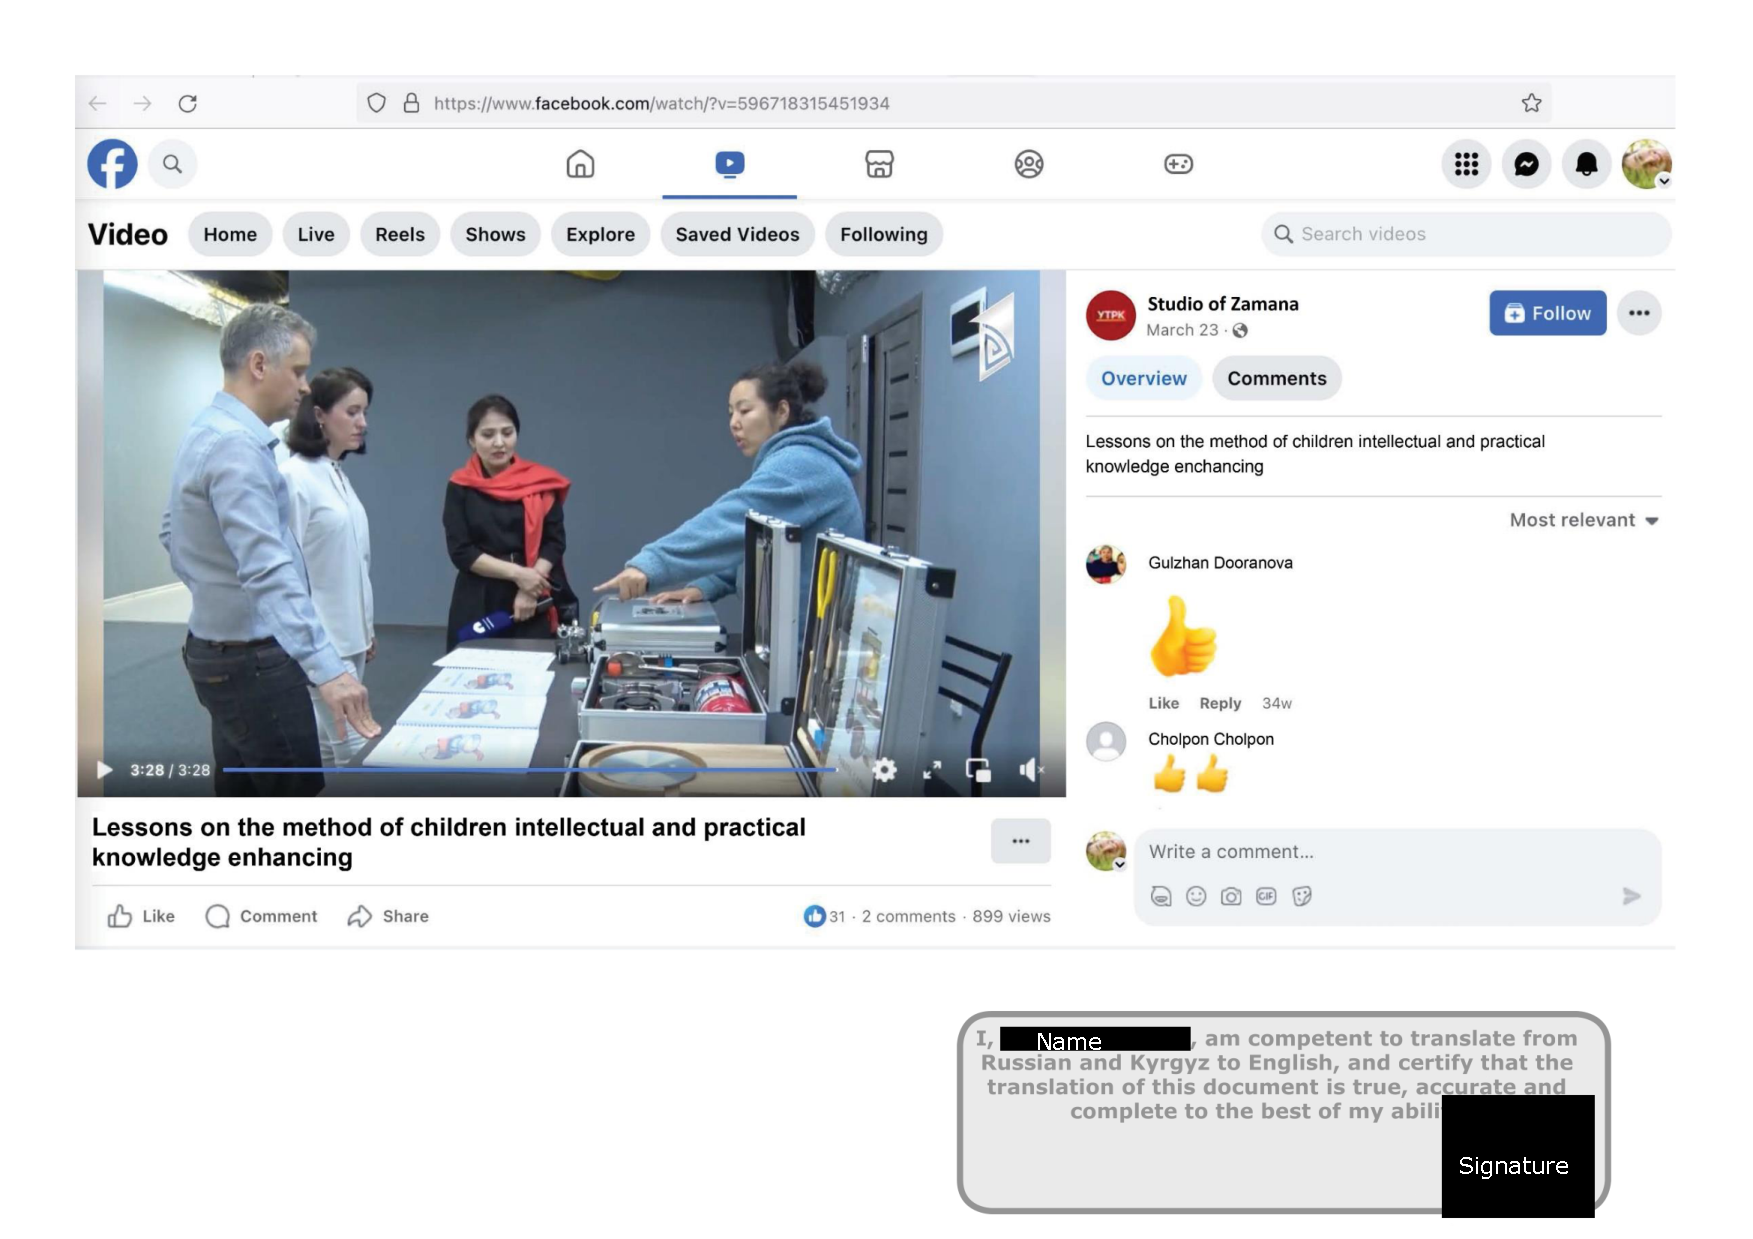
\includepdf[pages=-,angle=90]{3_28_stand_en_public}

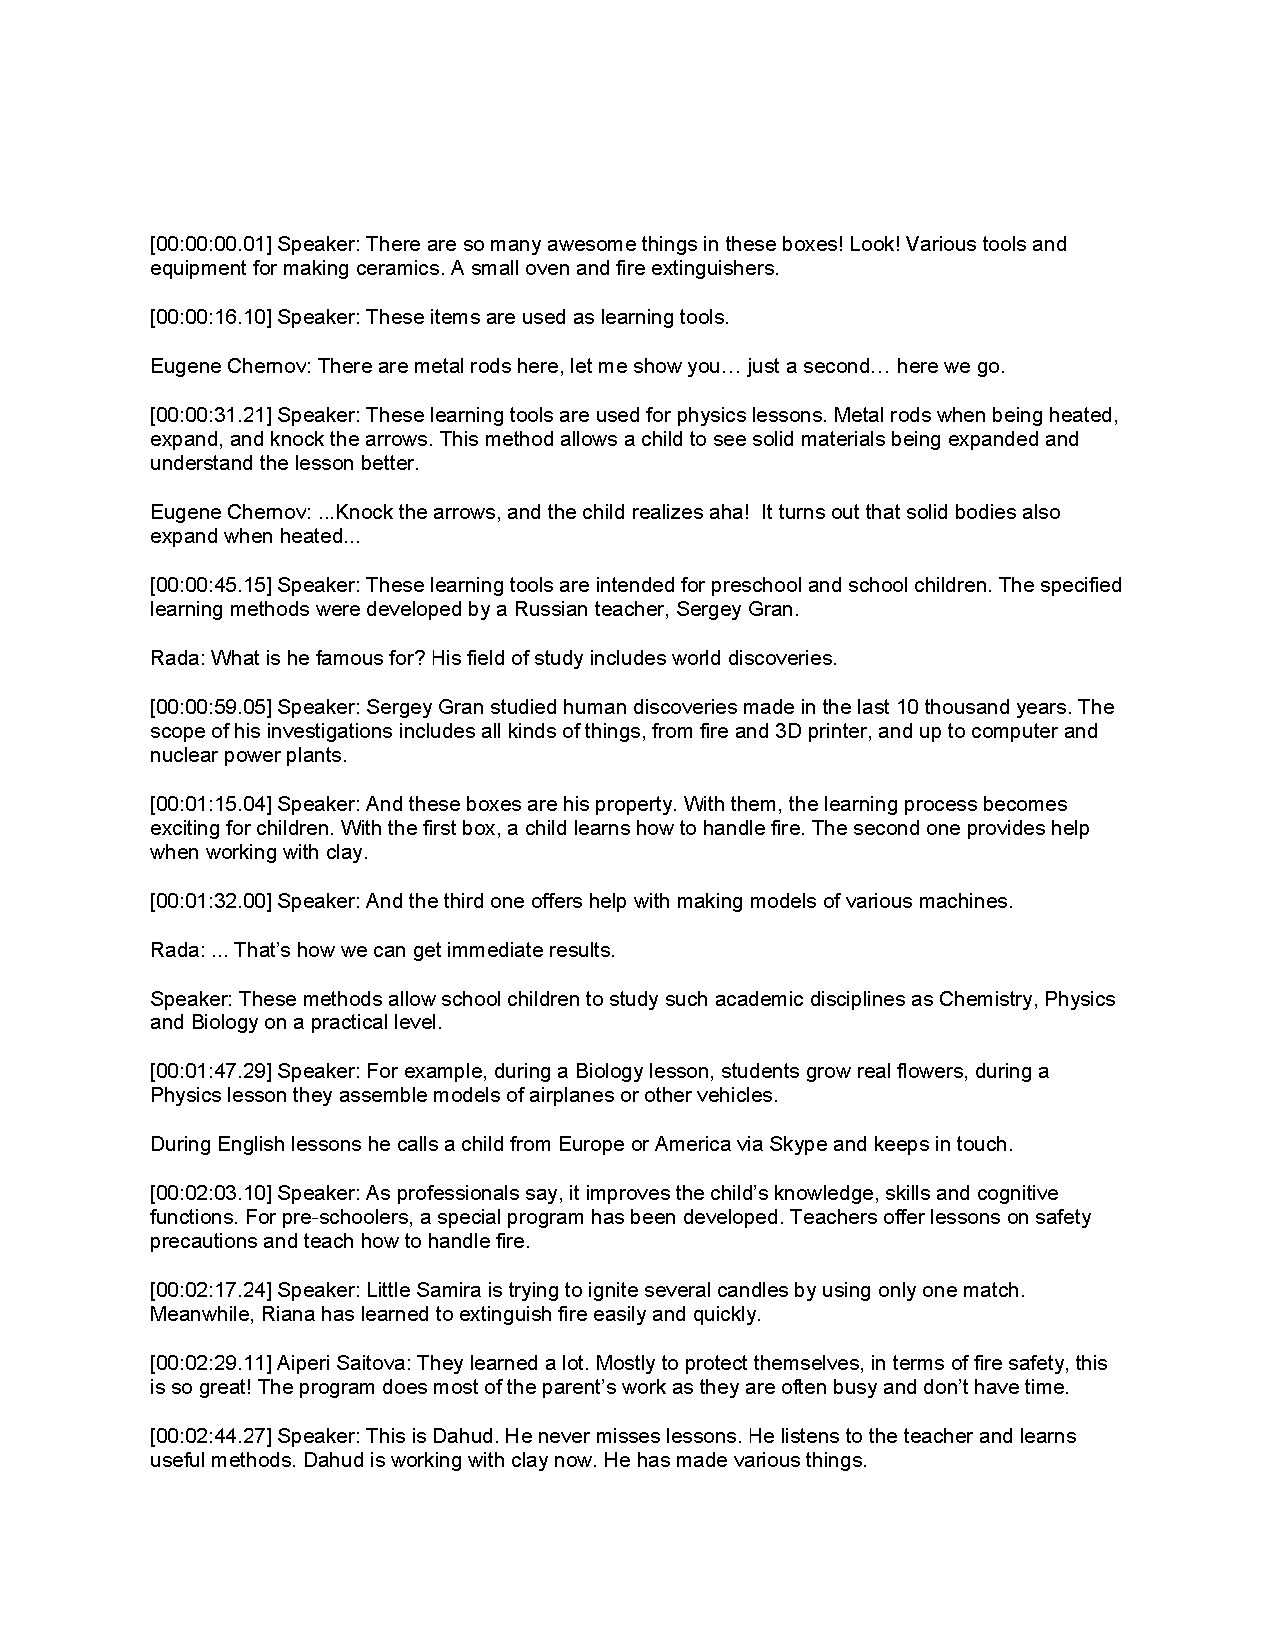
\includepdf[pages=-]{transcript_en_public}

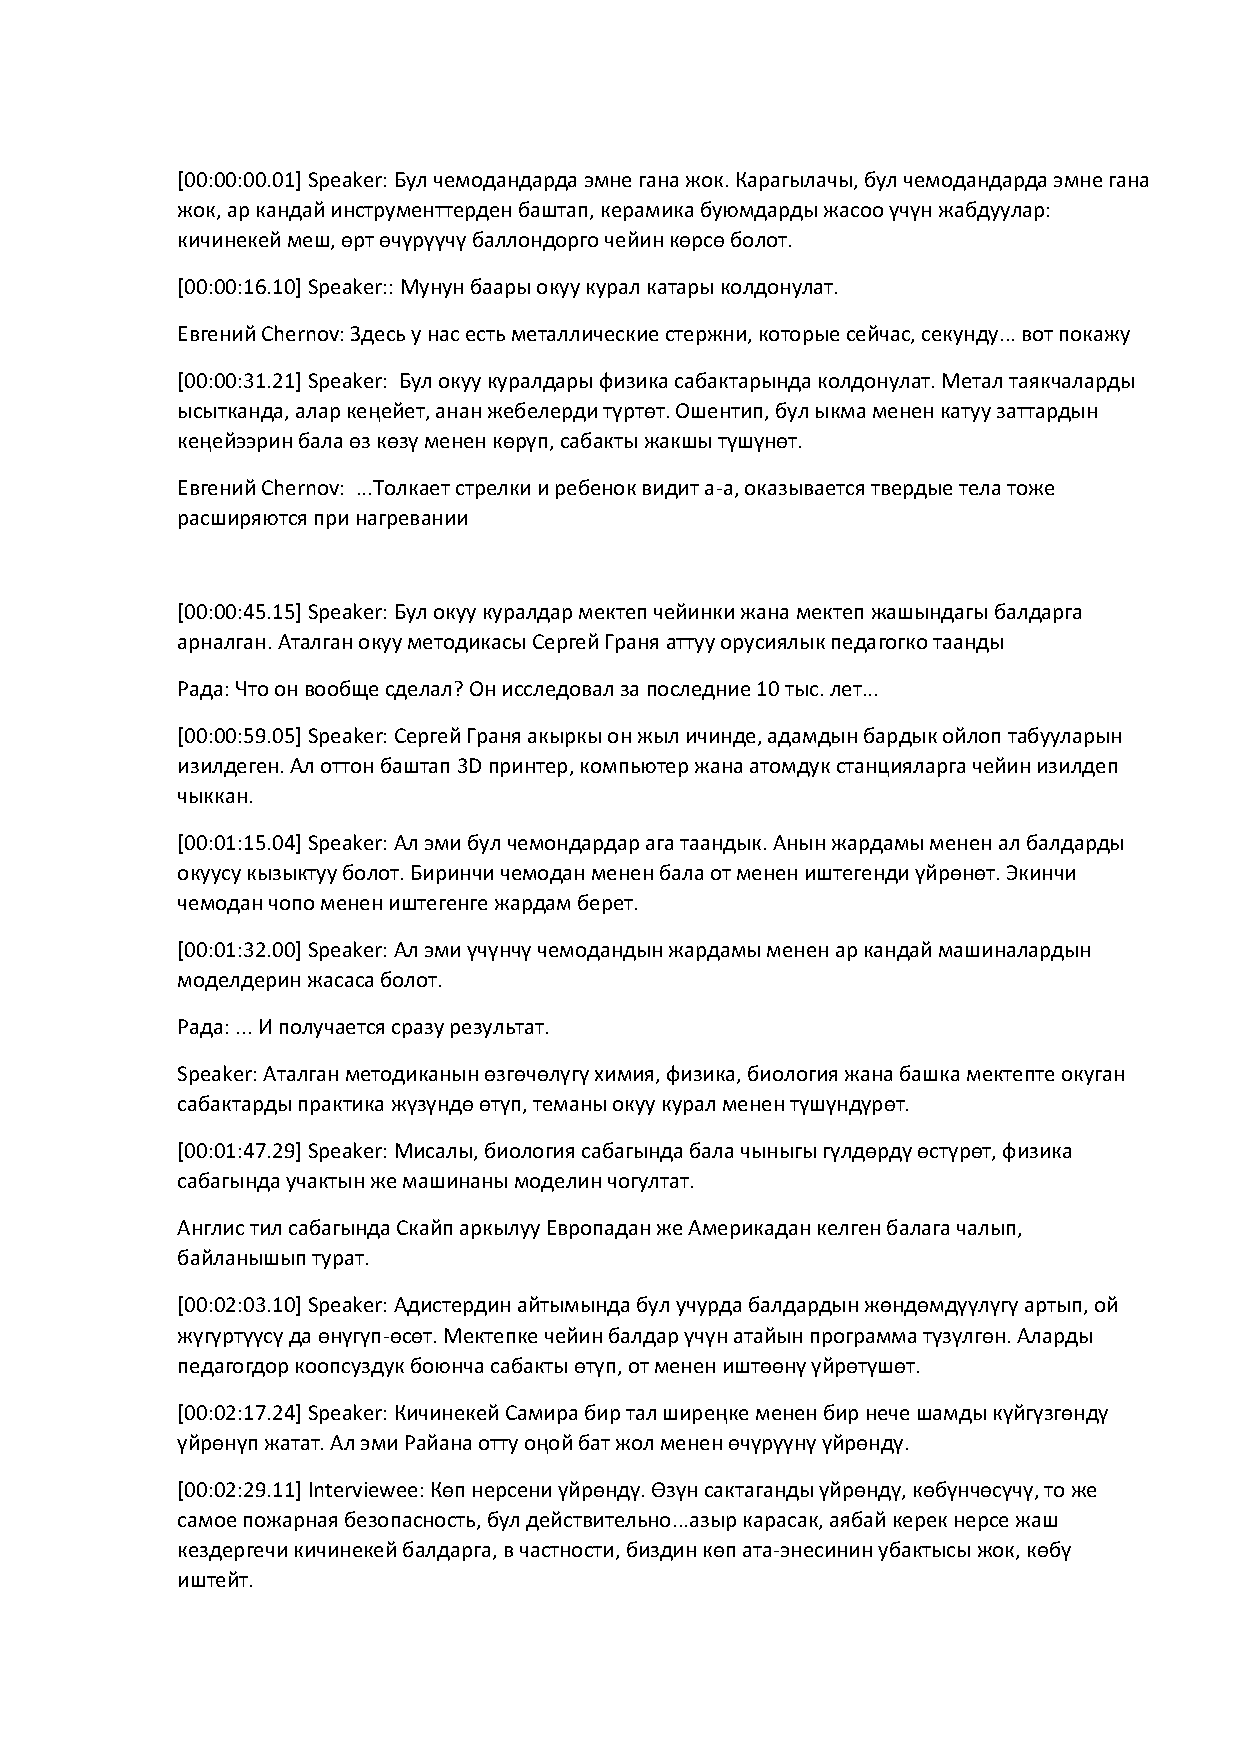
\includepdf[pages=-]{transcript}

\pagebreak
